\begin{question}
\noindent As part of a space exploration project, a science team is designing a small cuboid-shaped container to hold a Moon rock sample. The container has the dimensions shown below, all given in centimetres, in terms of $x$.

\begin{center}
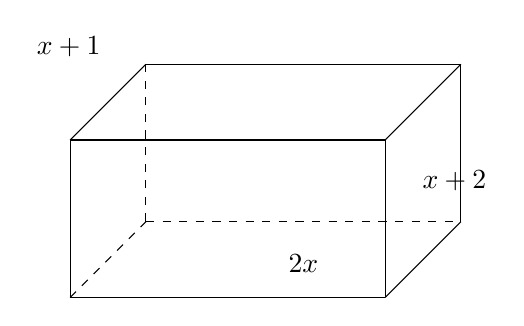
\begin{tikzpicture}[scale=1, transform shape]
    % Define the points of the cuboid
    \coordinate (A) at (0,0,0);
    \coordinate (B) at (0,0,-2.5);
    \coordinate (C) at (4,0,-2.5);
    \coordinate (D) at (4,0,0);
    \coordinate (A2) at (0,2,0);
    \coordinate (B2) at (0,2,-2.5);
    \coordinate (C2) at (4,2,-2.5);
    \coordinate (D2) at (4,2,0);

    % Draw the base (hidden edges dashed)
    \draw[dashed] (A) -- (B);
    \draw[dashed] (B) -- (C);
    \draw (C) -- (D);
    \draw (A) -- (D);

    % Draw the top
    \draw (A2) -- (B2);
    \draw (B2) -- (C2);
    \draw (C2) -- (D2);
    \draw (A2) -- (D2);

    % Draw the vertical edges
    \draw (A) -- (A2);
    \draw[dashed] (B) -- (B2);
    \draw (C) -- (C2);
    \draw (D) -- (D2);

    % Labels for dimensions
    \node at (2, -0.3, -2.5) [below] {$2x$};
    \node at (4.4, 1, -1.25) {$x+2$};
    \node at (-0.5, 2.7, -1.25) {$x+1$};
\end{tikzpicture}
\end{center}

\noindent The container is a cuboid with length $2x$ cm, width $(x+2)$ cm and height $(x+1)$ cm.

\begin{enumerate}
    \item[(a)] Show that the volume, $V$ cm$^3$, of the container is given by
    \[ V = 2x^3 + 6x^2 + 4x \]
    \vspace{4.5cm}
    \answermarks{3}

    \item[(b)] The scientists set $x = 5$ for the final design. Work out the volume of the container.
    \vspace{3cm}
    \answerunit{cm$^3$}{1}
\end{enumerate}
\end{question}